\chapter{Results}
\epigraph{``Another quote.''}{\vspace{10pt}Another author}
\label{chapter:results}
\newpage

This chapter presents the results obtained while evaluating the proposed algorithm/mechanisms. The discussion and analysis of results are presented in the \nameref{chapter:discussion} chapter.


\section{CNN as classifier}

\subsection{CNN acoustic location as classification}

The first evaluation of the CNN was on a clasification task where it had to classify the acoustic location of the sound source from the 26 possible locations, each one corresponding to a specific recording session characterized by the same X, and Y location and only changing the Z location. Trained on 20 epochs, the network shows a accuracy of 99.4\% on training and 98.59\% on the test set. The confusion matrix is shown in Figure \ref{fig:cnn_confusion_matrix}.

\begin{figure}[!htb]
    \begin{center}
        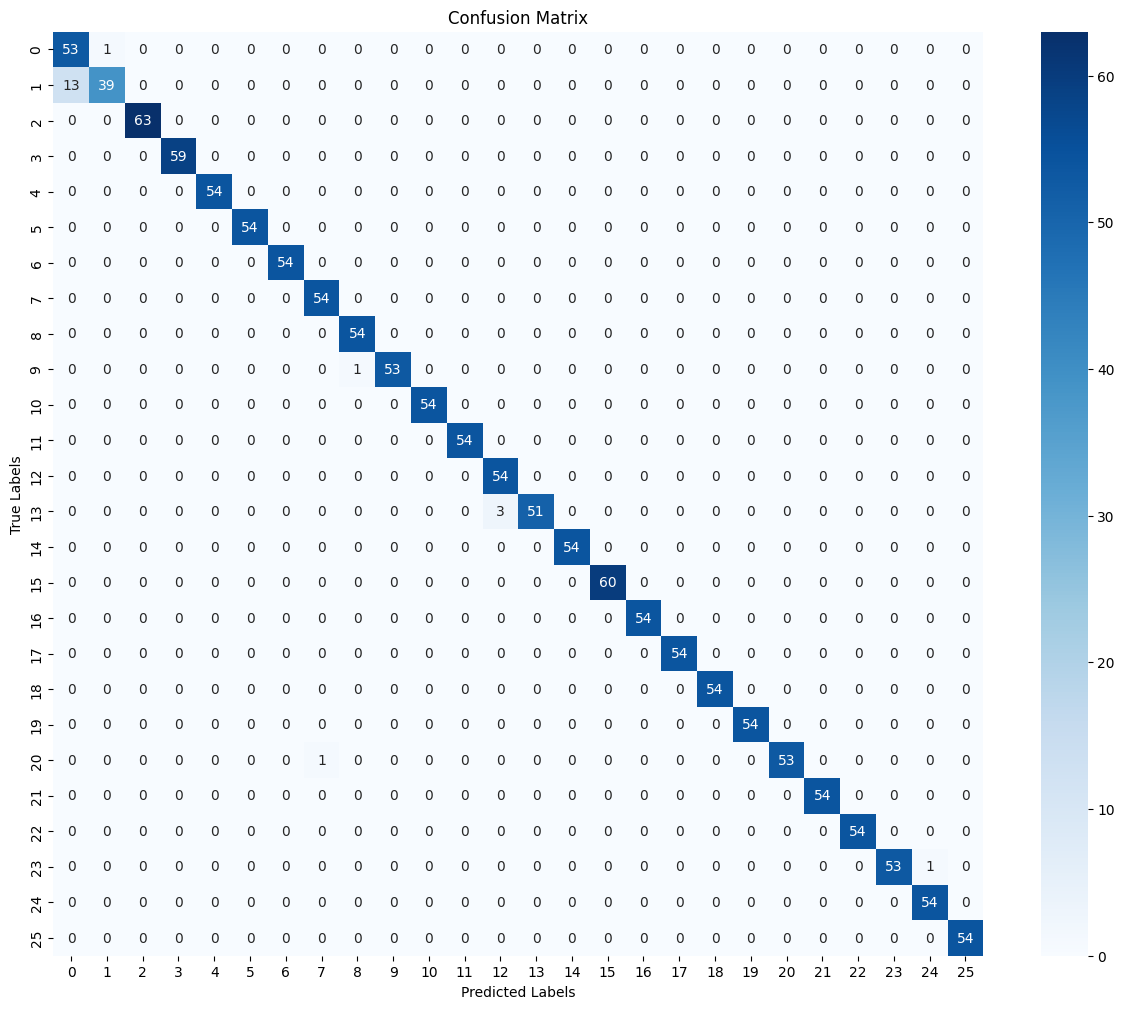
\includegraphics[height=12cm, width=13cm]{../img/clasification_location_cnn.png}
        \caption{Confusion matrix for CNN acoustic location classification on test set.}
        \label{fig:cnn_confusion_matrix}
    \end{center}
\end{figure}

\subsection{CNN acoustic orientation as classification}

The second evaluation of the CNN was on a clasification task where it had to classify based on the orientation of the cube from a total of 9 possible orientations. for each orientation the cube is rotated 10 degrees with respect to one of its centroidal axes. trained on 20 epochs, the network shows a accuracy of 99.0\% on training and 29.06\% on the test set. The confusion matrix is shown in Figure \ref{fig:cnn_confusion_matrix_orientation}.





\begin{figure}[!htb]
    \begin{center}
        \includegraphics[height=12cm, width=12cm]{../img/confusion_matrix_orientation_cnn.png}
        \caption{Confusion matrix for CNN acoustic orientation classification on test set.}
        \label{fig:cnn_confusion_matrix_orientation}
    \end{center}
\end{figure}

A further exploration is carried out to analyze the performance of the CNN on the orientation classification task. As shown in figure \ref{fig:session_points}, three regions are defined to reduce changes in orientation for the other Euler rotational axes. For each of the three regions,The accuracy results are presented in table and the corresponding confusion matrix  are presented in figure \ref{fig:cnn_confusion_matrix_orientation}. 

\begin{figure}[!htb]
    \begin{center}
        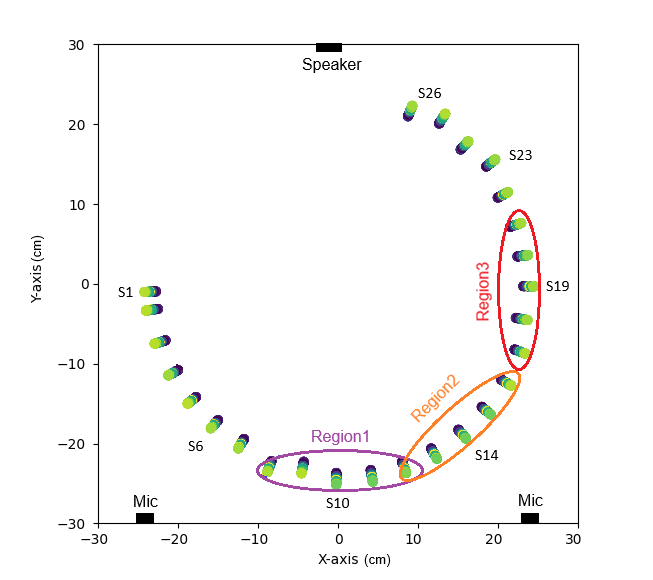
\includegraphics[height=12cm, width=12cm]{../img/cross-cor_points.png}
        \caption{Confusion matrix for CNN acoustic orientation classification on test set.}
        \label{fig:session_points}
    \end{center}
\end{figure}

Also to investigate the similarity of the acoustic signal when the cube is rotated or the cube is moved, a cross-correlation analysis was performed. The selected sessions for the analisis correspond to a sample that comprends diferent position that goes from the nearest to the mics to the farthest in the area near the speaker. The results of the cross-correlation analysis are presented in figure \ref{fig:cnn_confusion_matrix_orientation}. 

\begin{figure}[!htb]
    \begin{center}
        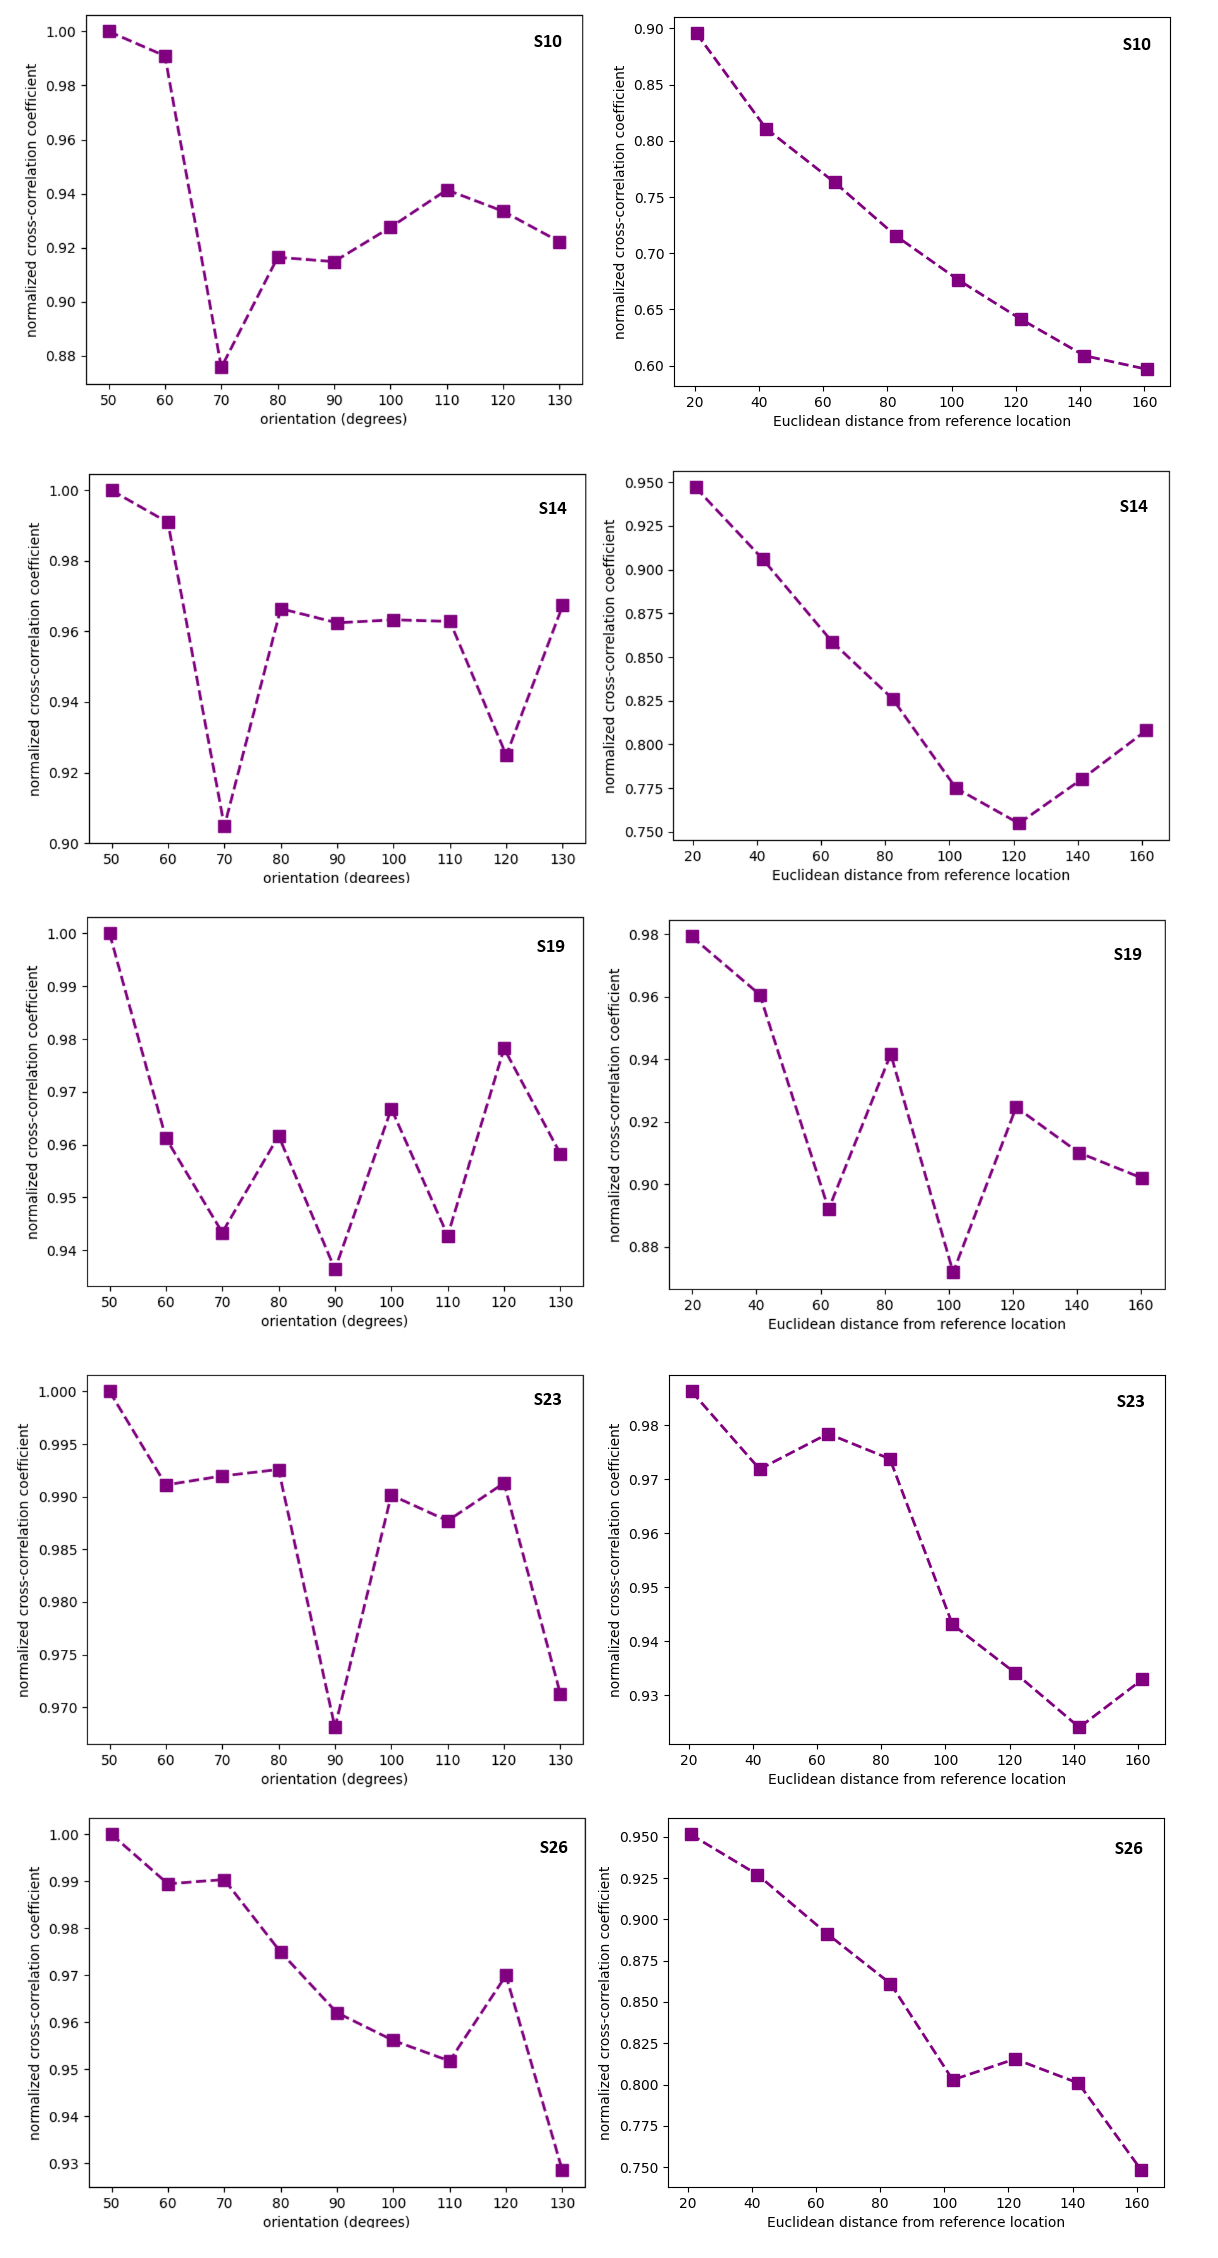
\includegraphics[height=20cm, width=13cm]{../img/reduced_allarround_xcor.png}
        \caption{Confusion matrix for CNN acoustic orientation classification on test set.}
        \label{fig:cnn_confusion_matrix_orientation}
    \end{center}
\end{figure}





\section{Statistical Tool Assumptions Tests}
The evaluation of the assumptions of the statistical tool used should be reported.

\section{Statistical Tool Results}
The results of the statistical tool used are presented in this section.

\section{Obtained Metrics}
Additional metrics obtained during the development of the research are presented in this section. 


\subsection{Most Complex Scenario Metrics (if needed)}


\section{Correctness (if needed)}
If the correctness of the proposal was evaluated, it should be presented in this section.
\section{Output (If needed)}
If the proposal's output differs from what was analyzed with the statistical tool, it should be presented in this section.
\newpage
